\documentclass[10pt,twocolumn,letterpaper]{article}
\usepackage[T1]{fontenc}
% Official CVPR 2026 style; this is a working manuscript, not a submission.
\usepackage[pagenumbers]{cvpr}
\usepackage[breaklinks,colorlinks,allcolors=blue]{hyperref}
\usepackage{array}
\usepackage{placeins}
\usepackage{algorithm}
\usepackage{algpseudocode}
\setcounter{dbltopnumber}{4}
\renewcommand{\dbltopfraction}{0.95}
\renewcommand{\dblfloatpagefraction}{0.15}
\makeatletter
\setlength{\@fptop}{0pt}
\setlength{\@fpsep}{14pt}
\setlength{\@fpbot}{0pt plus 1fil}
\makeatother
\def\confName{CVPR}
\def\confYear{2026}
\def\paperID{*****}
\begin{document}
\twocolumn[{%
\begin{center}
{\Large\bfseries BrickMore}\par\vspace{0.6em}
{\large Authors and affiliations to be added}\par\vspace{0.8em}
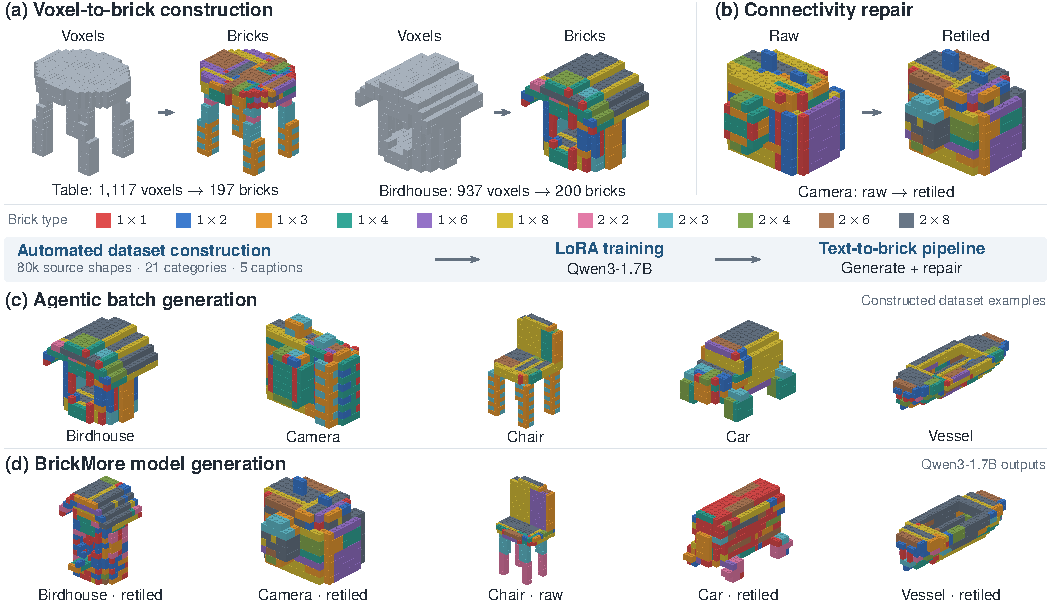
\includegraphics[width=\textwidth]{figure1.pdf}
\captionof{figure}{\textbf{BrickMore overview.} (a) Source voxels are converted into rectangular bricks. (b) Raw predictions are retiled to repair connectivity. (c) Examples from agentic batch generation of voxel data. (d) Outputs of the fine-tuned Qwen3-1.7B pipeline. Colors consistently encode brick type, independent of orientation; they are visualization labels, not predicted appearance. Voxels are shown in gray.}
\label{fig:teaser}
\end{center}\vspace{0.5em}
}]

\begin{abstract}
Generating brick structures from text is a geometric assembly problem: the layout must align with natural language and also place discrete pieces so that they fit in a bounded grid, connect through studs, and form a consistent structure. We present BrickMore, a text-to-brick framework that combines agentic batch generation of training data, language-model fine-tuning, and post-generation geometric repair in order to learn and constrain a spatial representation of brick assemblies. Using GPT-6.1 Sol, we develop an agentic batch-generation pipeline in which the model writes parametric generator programs that then produce three-dimensional voxel models in batches. The resulting shapes are converted into brick layouts through same-color tiling, connectivity analysis, and local bridging and retiling. The source dataset contains 80,000 voxel models across 21 object categories on a $48^3$ grid. Each model has five bilingual captions at different levels of detail, for 400,000 bilingual records in total. In the latest integrated version, 79,301 models pass the specified geometric checks. We fine-tune Qwen3-1.7B using low-rank adaptation (LoRA) on the English captions and brick-placement sequences, enabling it to predict brick dimensions and positions from text.

After generation, the pipeline forms a voxel union from the in-bounds portions of supported brick placements, uses mixed-integer linear programming (MILP) to seek an exact cover, and checks for a single stud-connected component. We evaluate the resulting structures against outputs from BrickGPT and BrickNet on 114 shared prompts. On the evaluated outputs, BrickMore achieves the highest mean scores across three text--image alignment metrics. It also obtains a mean invalid-placement ratio of 0.00\%, matching BrickGPT under the same metric. These comparisons use a shared rendering protocol.

\end{abstract}
\section{Introduction}
Text-to-three-dimensional generation enables users to describe and create objects using natural language. Generating brick structures adds the requirement that a target shape be represented as discrete pieces and their spatial placements. In addition to matching the text, the resulting structure must account for overlaps and connections between bricks: a layout may resemble the described object while containing intersecting bricks or disconnected parts, and thus fail to meet the specified geometric requirements. The setting is therefore one of geometric reasoning and object assembly: the system must decide how bricks fit, interlock, and remain connected in space, not only whether the overall shape resembles the described object.

Prior work has explored text-driven brick generation through different representations and generation constraints. BrickGPT trains an autoregressive language model on paired text and brick structures and applies validity checks and physics-aware rollback during inference (Pun et al., 2025)~\cite{brickgpt}. BrickNet uses a graph-based representation to generate assembly sequences involving a broader range of parts and connection types (Kulits and Schmid, 2026)~\cite{bricknet}. These works demonstrate the importance of structural representations and generation constraints for brick modeling.

For voxel-based shapes, spatial adjacency between voxels does not necessarily imply a valid connection between bricks. A voxel shape can form a connected volume even when the bricks covering it only touch side by side without stud connections. This distinction affects both data construction and generation: converting voxel shapes into training targets requires attention to coverage and brick connectivity, while predicted layouts may also contain overlaps or disconnected components that require further processing.

To study this problem, we present BrickMore. Using GPT-6.1 Sol, we develop an agentic batch-generation pipeline: the model writes parametric generator programs, which then produce voxel models in batches, and we convert the resulting models into brick layouts. The source dataset contains 80,000 models across 21 object categories, represented on a $48^3$ grid, with five bilingual captions for each model. We tile occupied voxels with same-color rectangular bricks and combine connection analysis with local bridging and retiling to address ungrounded components. Some derived targets involve limited changes to the source voxels; these changes and the original data are recorded separately. In the latest integrated version, 79,301 models pass the specified geometric checks.

We fine-tune Qwen3-1.7B with LoRA on English captions and brick-placement sequences. Given a text prompt, the model predicts brick dimensions and positions; the current output does not include color. To address potential overlaps and connectivity defects, we form a target union from the in-bounds voxels of supported brick placements, use MILP to seek an exact cover, and check for a single stud-connected component. For some cases in which no feasible layout is found within the solver's time budget, the system regenerates a sequence using a different language-model sampling seed. The training data use a $48^3$ workspace, multi-level captions, and a fixed spatial serialization of placements; conversion-time geometric checks and post-generation exact-cover retiling further constrain coverage, overlaps, and stud connectivity. The connectivity check is geometric; physical stability and the feasibility of an assembly order require separate evaluation.

To evaluate the resulting structures, we compare the provided outputs of BrickMore, BrickGPT, and BrickNet on 114 shared prompts across 21 object categories and five description levels. We measure text--image alignment using VQAScore, PE, and SigLIP2, and evaluate the proportion of invalid brick placements using $P_{\mathrm{inv}}$. Under a common rendering protocol, BrickMore achieves the highest mean scores on all three text--image metrics. BrickMore and BrickGPT both obtain a mean $P_{\mathrm{inv}}$ of 0.00\% when evaluated in file order. These results describe the provided outputs under the specified evaluation protocol and do not independently establish physical stability or assembly feasibility.

Our contributions are as follows:

\begin{enumerate}
\item We develop an automated $48^3$ voxel data-generation pipeline by agentic batch generation with GPT-6.1 Sol, which writes parametric generator programs that produce 80,000 source models across 21 categories, each with five bilingual captions. In the latest integrated version, 79,301 models pass the specified geometric checks. This data-generation process supplies geometrically checked layouts for fine-tuning a text-conditioned spatial representation of brick assemblies.
\item We develop a voxel-to-brick conversion pipeline that combines same-color tiling, connection analysis, and local bridging and retiling, while recording limited changes to source voxels in derived targets, so that training targets encode stud-connected assemblies rather than voxel adjacency alone.
\item We fine-tune Qwen3-1.7B for text-to-brick generation and combine it with a post-generation pipeline based on voxel unions, exact-cover MILP, and connectivity checks. This is a fine-tuning and geometric-repair pipeline for text-to-assembly generation.
\end{enumerate}
% Queue this double-column figure early so it appears on page 3.
\begin{figure*}[t]
\centering
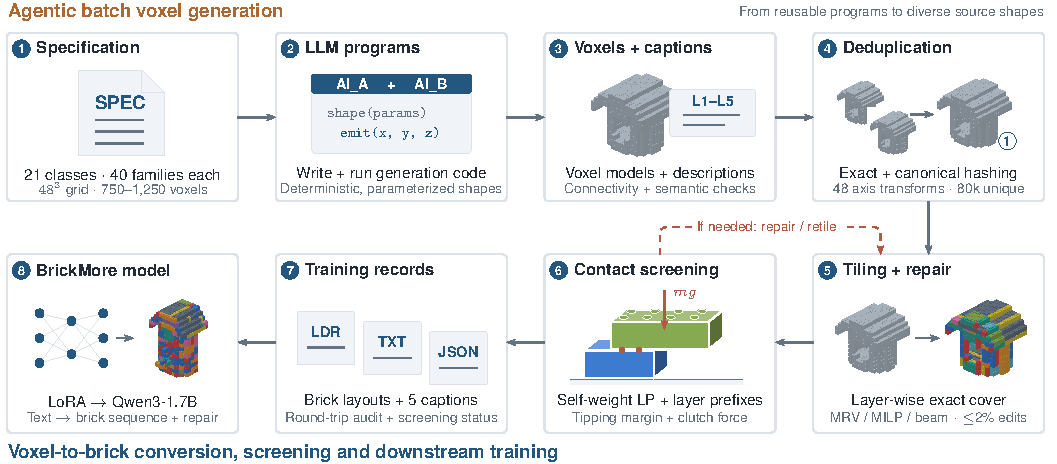
\includegraphics[width=\textwidth]{figure2.pdf}
\caption{\textbf{Visual data-construction workflow.} Parametric programs written by GPT-6.1 Sol through agentic batch generation produce voxel shapes and descriptions, followed by deduplication, voxel-to-brick tiling, repair, contact-based screening, and audited export for downstream fine-tuning. The dashed arrow denotes repair or retiling when needed. This diagram summarizes the historical construction workflow; screening is distinct from a guarantee of physical stability. Brick colors follow the type legend in Figure~\ref{fig:teaser}.}
\label{fig:data-workflow}
\end{figure*}
\section{Related Work}
Text-to-brick generation. BrickGPT represents a design as an autoregressively generated sequence of brick placements and uses brick-level rejection sampling together with physics-aware rollback during inference (Pun et al., 2025)~\cite{brickgpt}. BrickNet instead represents part connectivity through a graph-backed parametrization and trains autoregressive models on its assembly sequences (Kulits and Schmid, 2026)~\cite{bricknet}. BrickMore also generates placement sequences from text, then examines geometric reconstruction and connectivity in a separate post-generation stage.

Stability analysis. StableLego studies the structural stability of block-stacking assemblies using an optimization formulation based on force balance (Liu et al., 2024)~\cite{stablelego}. Such analyses depend on their mechanical assumptions. In BrickMore, geometric connectivity and the contact-based screening described in the dataset materials address different properties; neither alone establishes that every generated model can be physically assembled and remains stable.

\section{Dataset Construction}
\subsection{Parametric Voxel Generation}
The source dataset contains 80,000 voxel models on a $48^3$ grid across 21 object categories. Each model is paired with five bilingual captions at different levels of detail. The models are produced by parametric generator programs written through an agentic batch-generation process with GPT-6.1 Sol; the programs, rather than the language model itself, emit the voxel coordinates in batches. Each model record includes a geometry plan and a dataset version identifier to support reproduction.

\begin{figure*}[t]
\centering
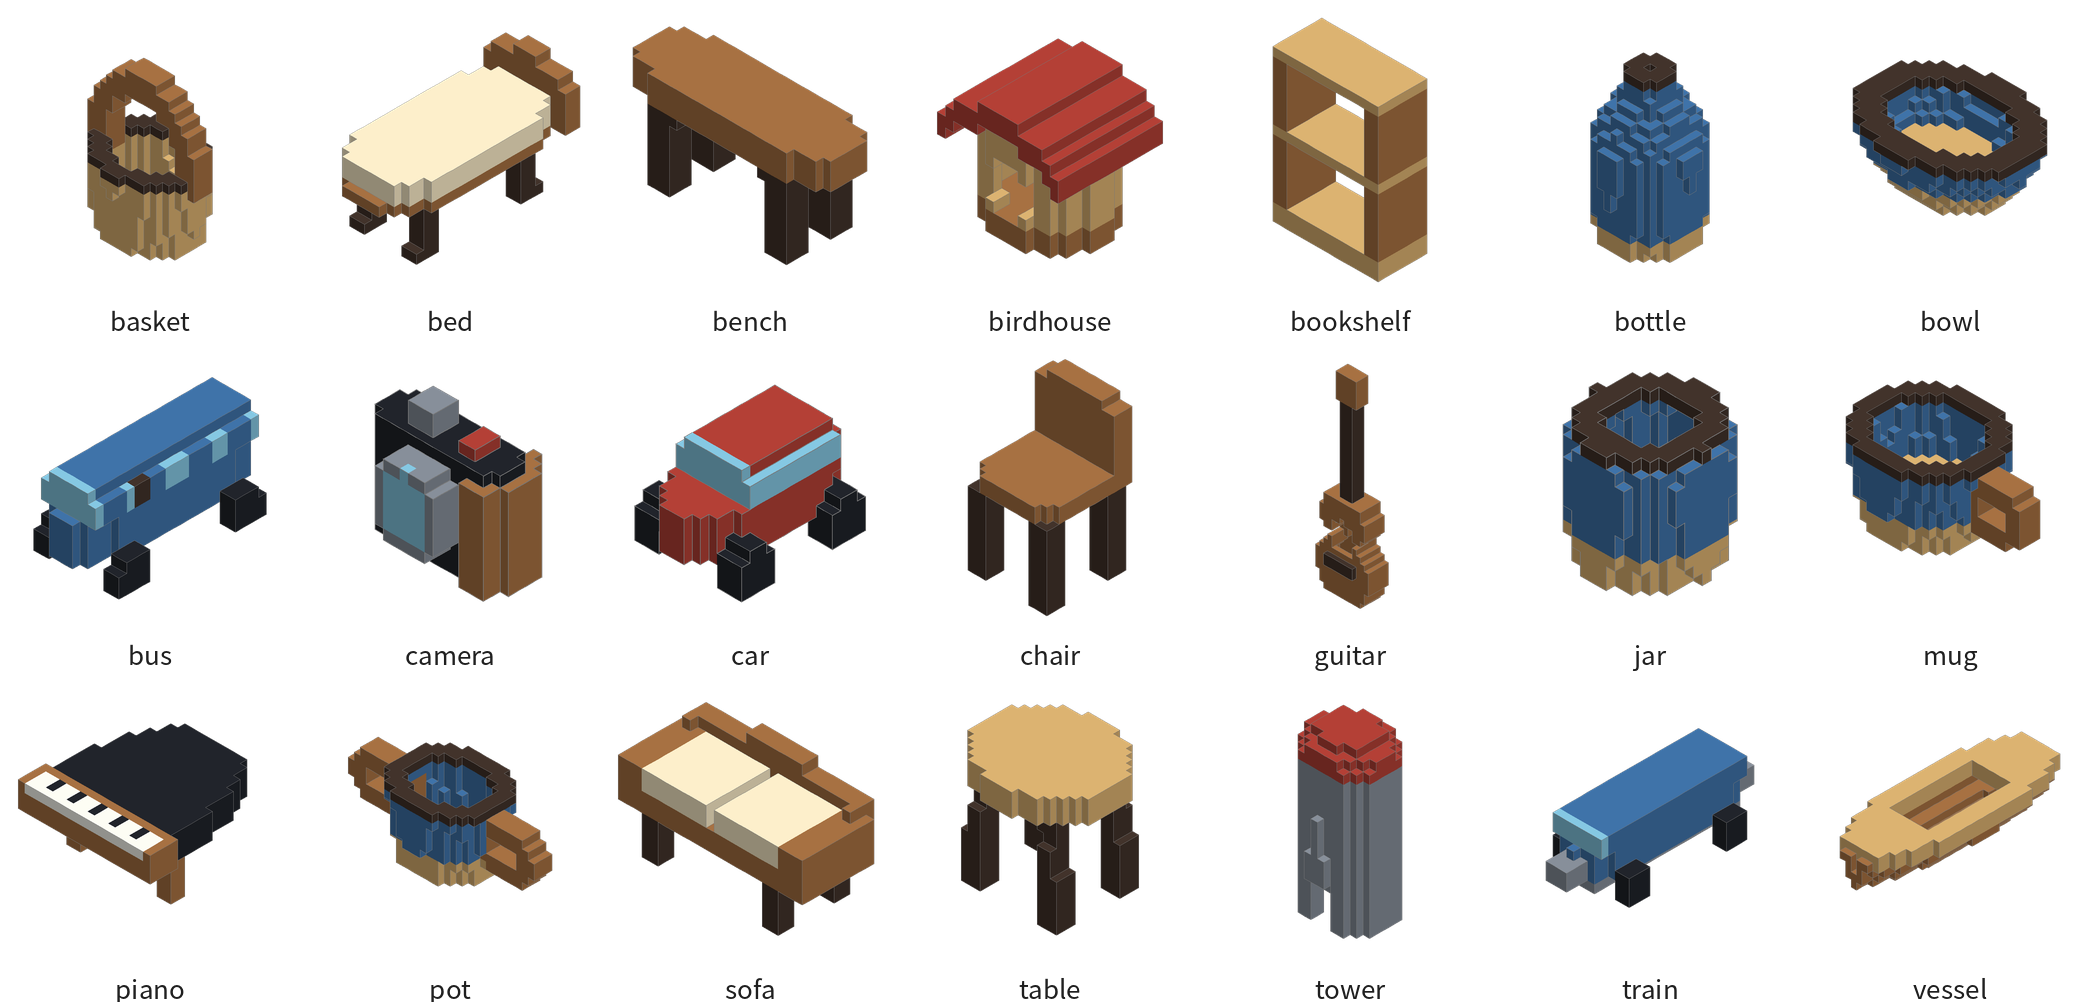
\includegraphics[width=0.475\textwidth,height=0.15\textheight,keepaspectratio]{figures/image7.png}\hfill
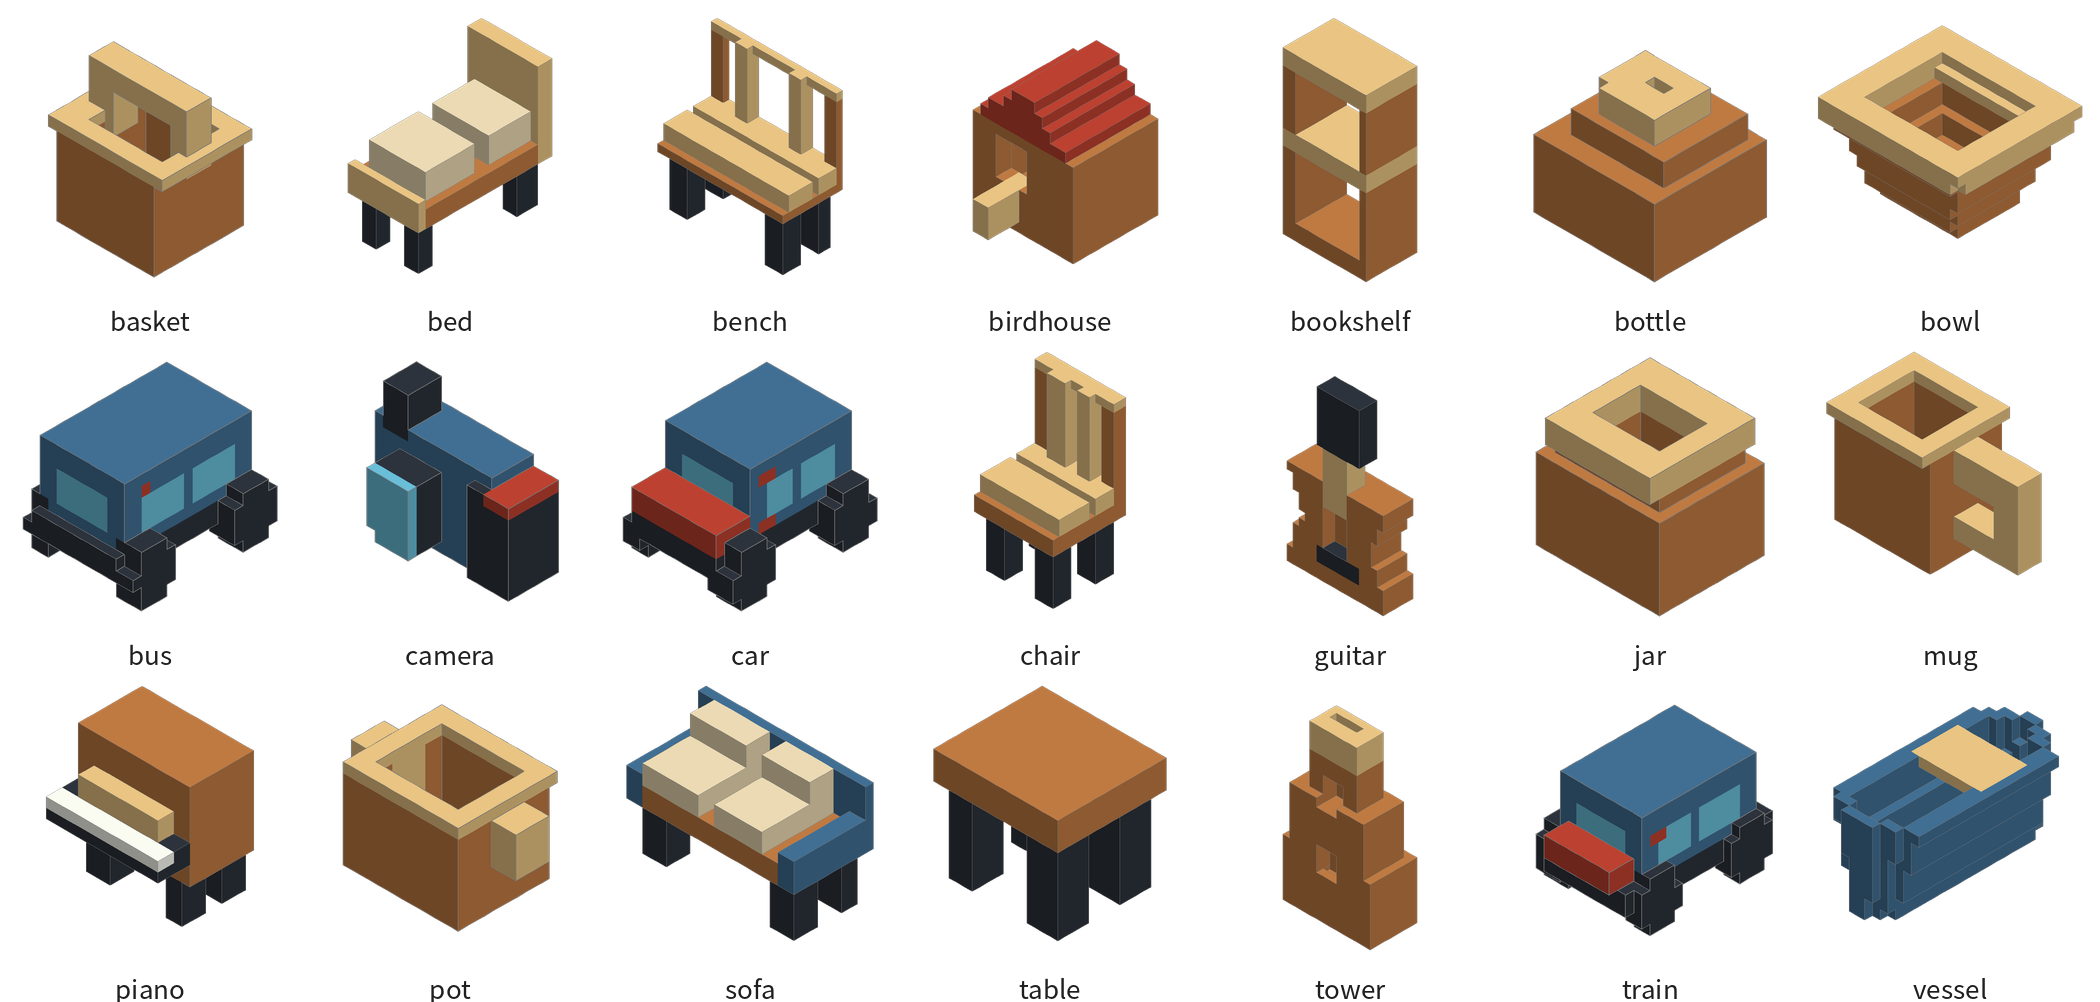
\includegraphics[width=0.475\textwidth,height=0.15\textheight,keepaspectratio]{figures/image8.png}\\
\caption{Voxel model samples from the reference document, spanning 21 object categories.}
\end{figure*}

\subsection{Voxel-to-Brick Conversion}
The conversion pipeline tiles occupied voxels with same-color rectangular bricks and analyzes their connections. Local bridging and retiling are used to address ungrounded components, with changes to source voxels recorded separately. The historical relaxed and retile dataset variants may contain multiple components that are individually grounded; this criterion differs from the single-component check used in the post-generation pipeline.

\begin{figure*}[t]
\centering
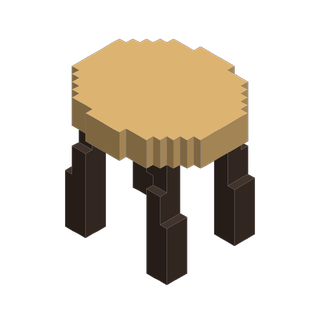
\includegraphics[width=0.2375\textwidth,height=0.15\textheight,keepaspectratio]{figures/image4.png}\hfill
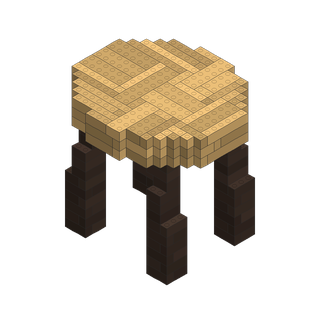
\includegraphics[width=0.2375\textwidth,height=0.15\textheight,keepaspectratio]{figures/image5.png}\hfill
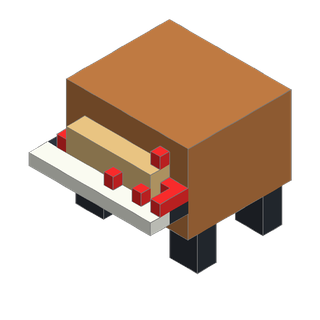
\includegraphics[width=0.2375\textwidth,height=0.15\textheight,keepaspectratio]{figures/image2.png}\hfill
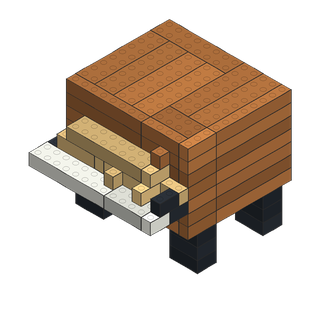
\includegraphics[width=0.2375\textwidth,height=0.15\textheight,keepaspectratio]{figures/image3.png}\\
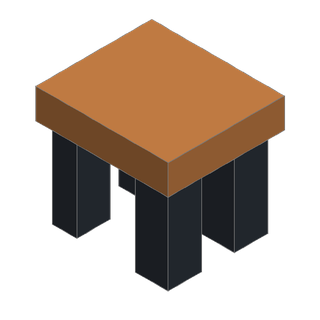
\includegraphics[width=0.2375\textwidth,height=0.15\textheight,keepaspectratio]{figures/image9.png}\hfill
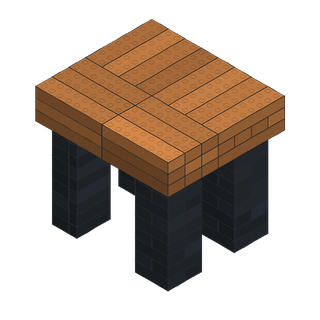
\includegraphics[width=0.2375\textwidth,height=0.15\textheight,keepaspectratio]{figures/image10.png}\hfill

\includegraphics[width=0.2375\textwidth,height=0.15\textheight,keepaspectratio]{figures/image11.png}\hfill
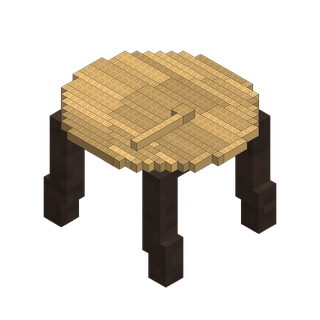
\includegraphics[width=0.2375\textwidth,height=0.15\textheight,keepaspectratio]{figures/image12.png}\\
\caption{Historical examples of voxel targets and brick layouts after local repair.}
\end{figure*}

\subsection{Geometric Checks and Physical Screening}
Geometric checks assess properties of the constructed layout under the relevant release rules. The reference materials also describe a contact-based gravity screening procedure under specified assumptions. Its outputs are screening results rather than proof of full physical stability; assumptions, coverage, and status counts for the exact dataset version require verification before being reported as final results.

\begin{figure*}[t]
\centering
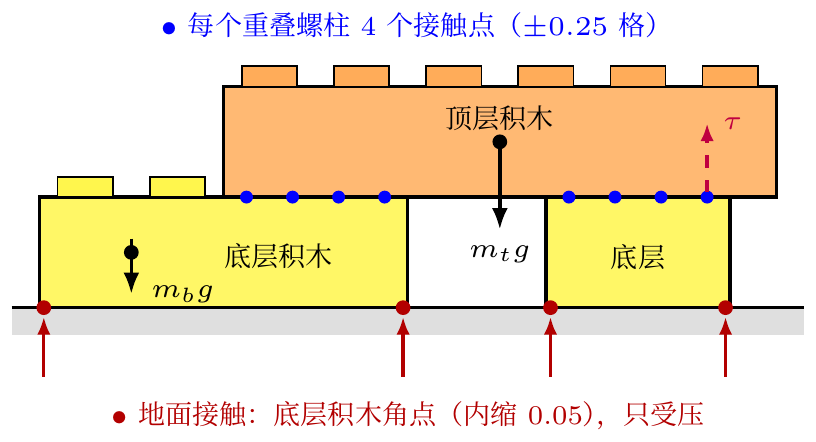
\includegraphics[width=0.88\textwidth,height=0.34\textheight,keepaspectratio]{figures/image13.png}\\[-0.3em]
\caption{Illustration of the historical contact-based gravity screening model; source labels are retained.}
\end{figure*}

\subsection{Dataset Output and Audit}
The historical full retile report records 79,298 geometrically passing models. Replacing the original 1,905 batch-B piano slots, of which 1,902 passed, with the updated release containing 1,905 passing models yields an integrated accounting of 79,301 passing models. This number is computed from the two release reports; it is not a new full-dataset verification run. The original A/B download procedure does not automatically perform this replacement.

\section{Dataset Statistics and Analysis}
\begin{table*}[t]\centering\small\begin{tabular}{lr}\toprule
Item & Value \\ \midrule
Source models & 80,000 \\
Categories & 21 \\
Grid & $48^3$ \\
Bilingual caption records & 400,000 (five per model) \\
Historical retile geometry passes & 79,298 / 80,000 \\
Integrated accounting & 79,301 / 80,000 \\
\bottomrule\end{tabular}\caption{Dataset statistics and version boundaries.}\end{table*}
The historical and integrated figures represent different version boundaries. The rules used by each release and the source of the integrated figure should accompany any comparison. Section~\ref{sec:training} uses the integrated 79,301-model corpus for fine-tuning on English captions.

\begin{figure*}[t]
\centering
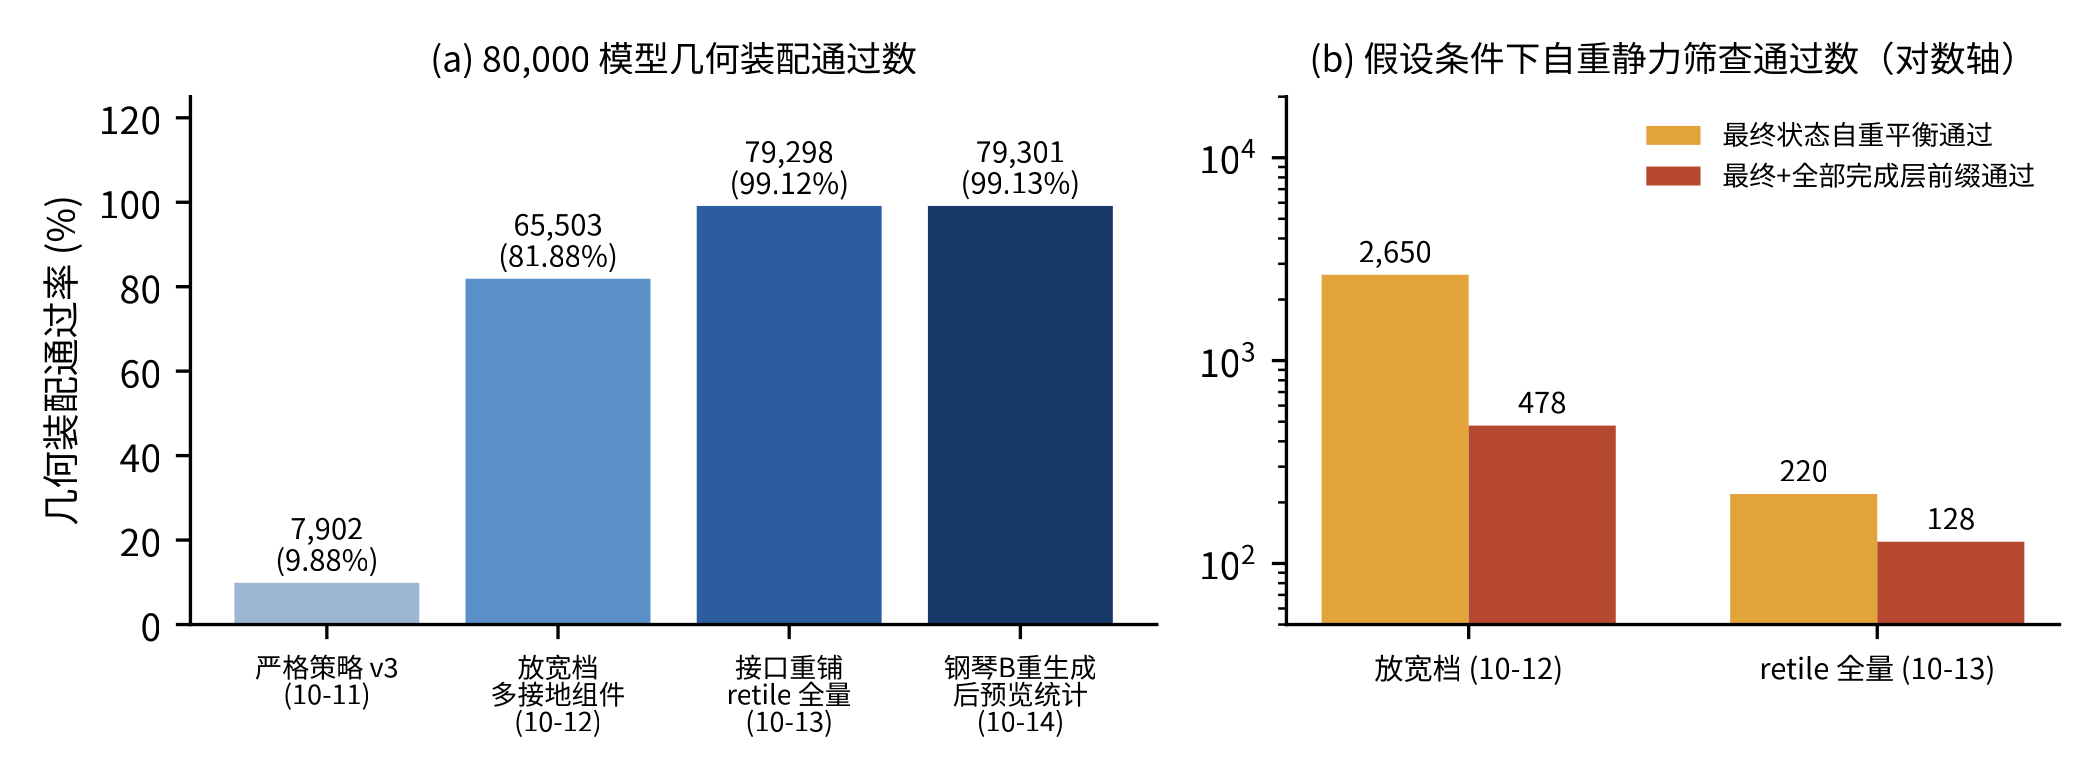
\includegraphics[width=0.88\textwidth,height=0.34\textheight,keepaspectratio]{figures/image14.png}\\[-0.3em]
\caption{Historical comparison of geometric conversion and screening outcomes. Version and numerical labels require verification.}
\end{figure*}

\begin{figure*}[t]
\centering
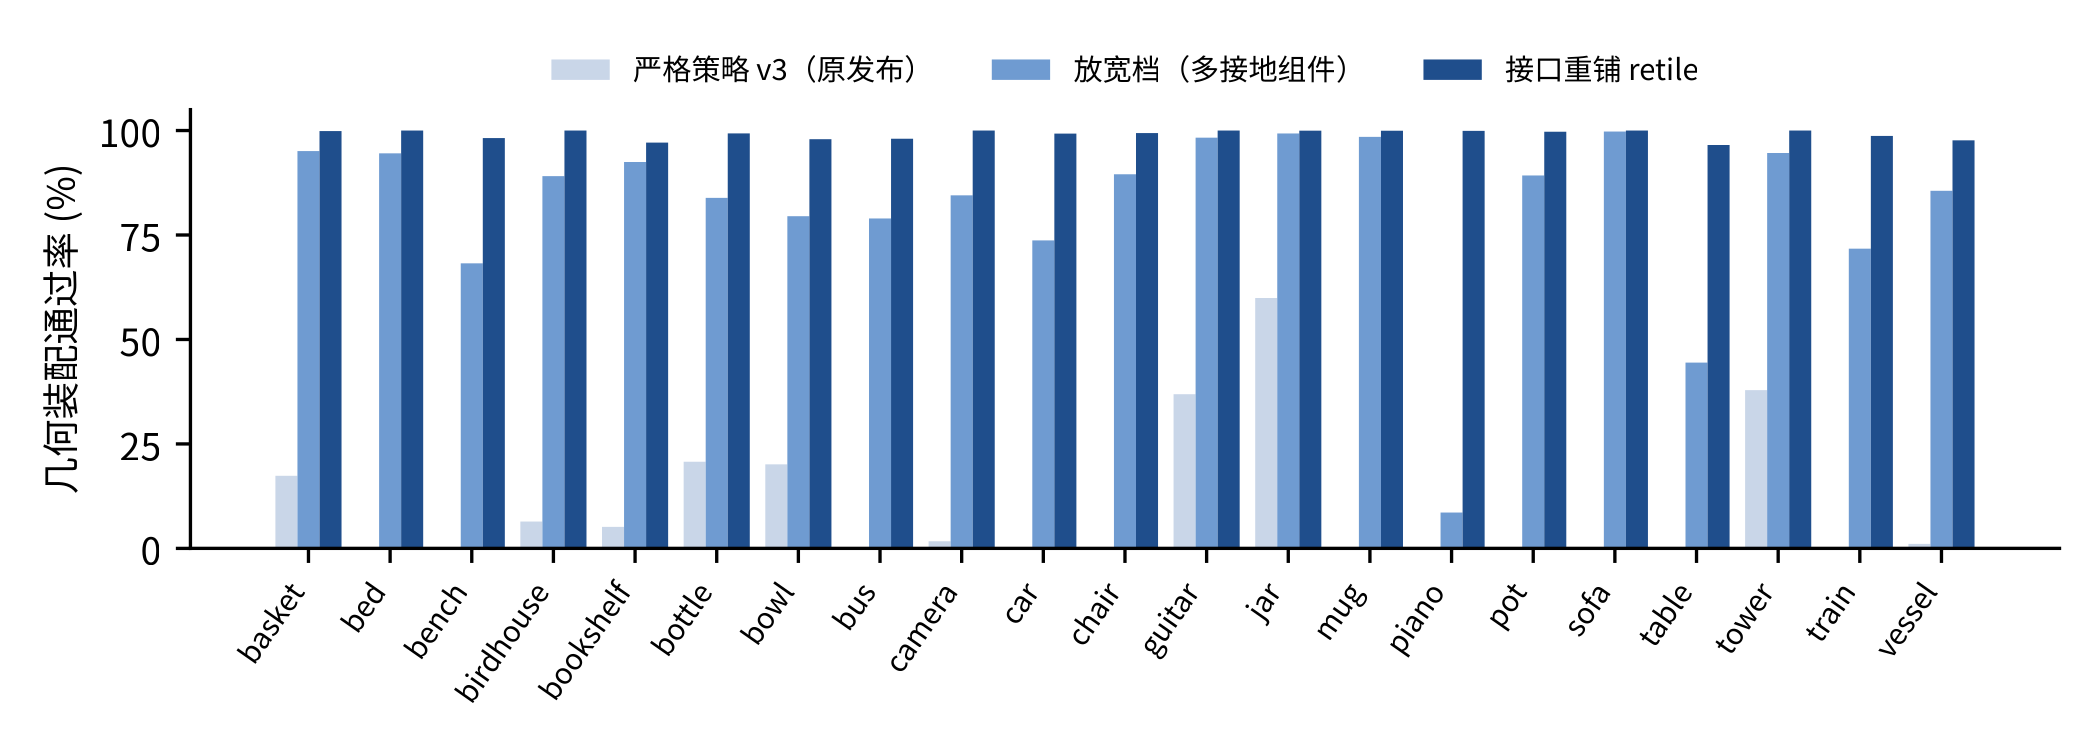
\includegraphics[width=0.88\textwidth,height=0.34\textheight,keepaspectratio]{figures/image15.png}\\[-0.3em]
\caption{Historical category-level geometric pass rates. Version and numerical labels require verification.}
\end{figure*}

\begin{figure*}[t]
\centering
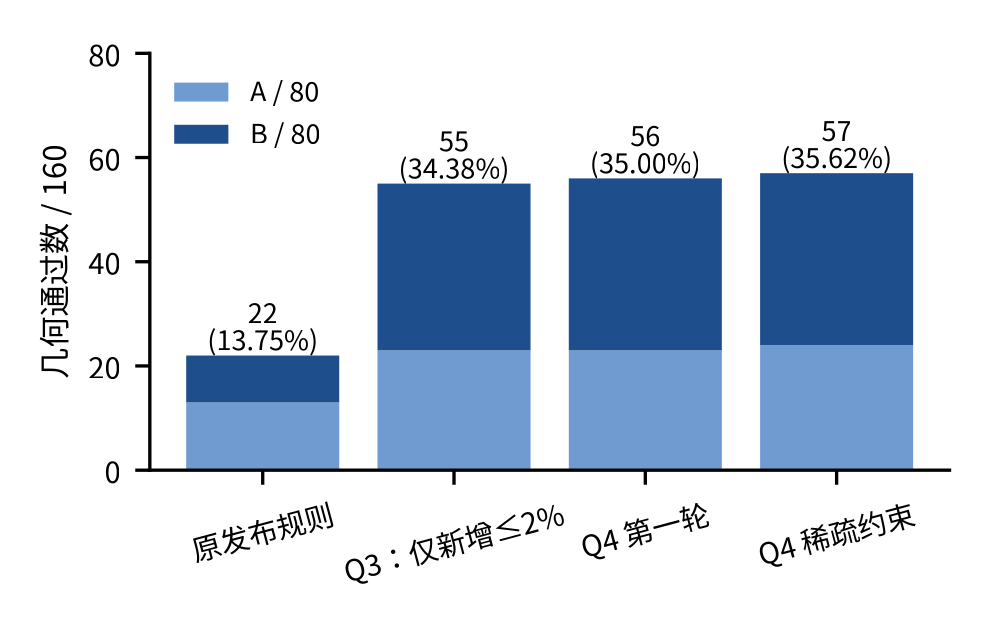
\includegraphics[width=0.88\textwidth,height=0.34\textheight,keepaspectratio]{figures/image16.png}\\[-0.3em]
\caption{Historical results on a 160-model sample. Version and numerical labels require verification.}
\end{figure*}

\subsection{Physical Screening Results}
Physical screening results are kept separate from geometric pass rates. Assumptions, assessed sample counts, and unresolved cases belong with the specific release being reported; historical counts from different releases are not combined here without a version-matched audit.

\begin{figure*}[t]
\centering
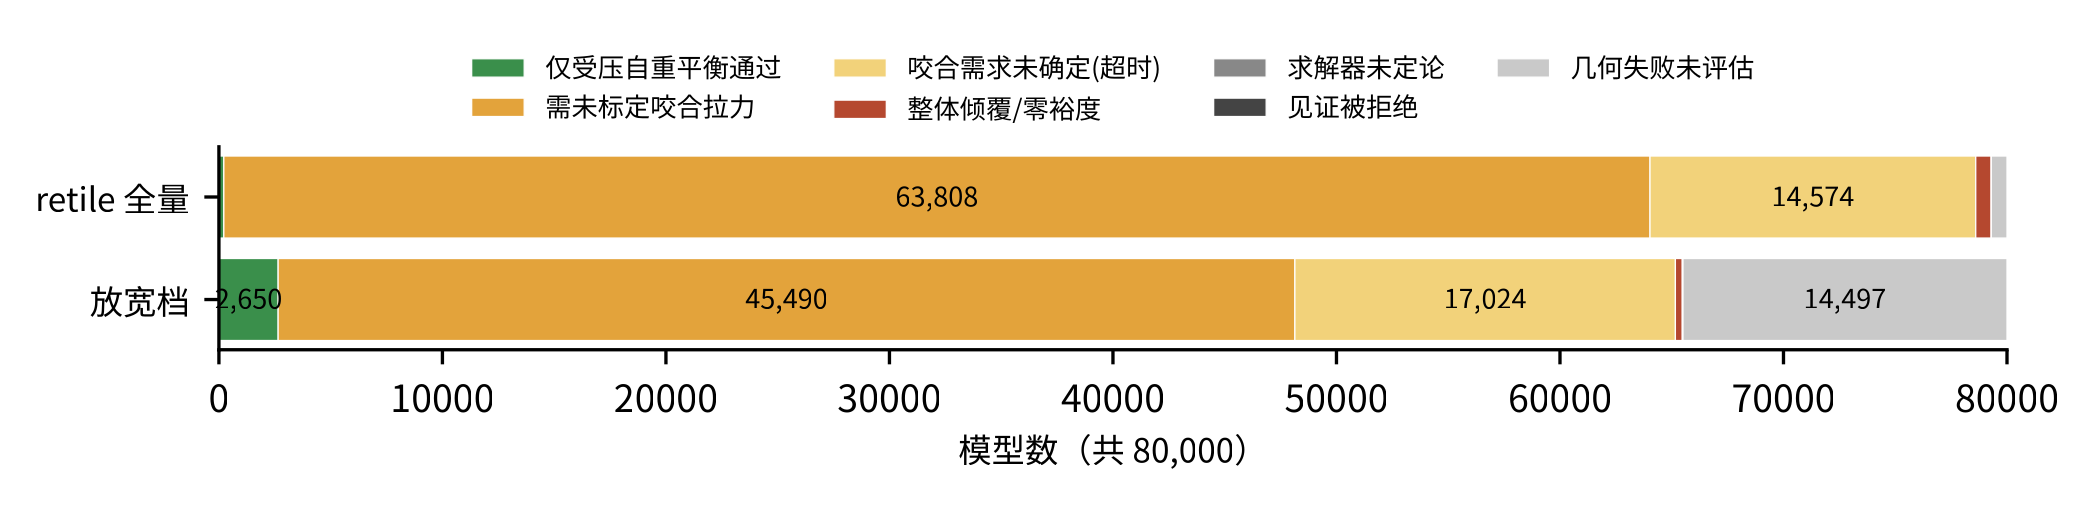
\includegraphics[width=0.88\textwidth,height=0.34\textheight,keepaspectratio]{figures/image17.png}\\[-0.3em]
\caption{Historical distributions of physical screening statuses. Counts refer to the specific releases shown.}
\end{figure*}

\section{BrickMore-48 Text-to-Brick Model}
We fine-tune Qwen3-1.7B using LoRA on English captions and brick-placement sequences. Given a text prompt, the model predicts dimensions and positions of bricks. The current output does not include color. The training corpus, model-level split, and fine-tuning configuration are described in Section~\ref{sec:training}.

Inference follows a seed-escalation and post-generation repair procedure, summarized in Algorithm~\ref{alg:inference-retiling}. The model samples a placement sequence with thinking disabled, temperature $0.7$, top-$p$ $0.9$, and a limit of $8192$ new tokens, using seeds $42$, $104$, and $2026$ in that order. A candidate is accepted when generation completes and the geometry validator reports no errors. If no such candidate exists, the pipeline keeps the completed draft with the fewest validator error records, denoted $\mathrm{Err}(\cdot)$, which counts line-format, library-membership, bounds, and overlap errors. It then forms a voxel union from the in-bounds cells of supported library placements, solves a shape-preserving exact cover with a single stud-connected component using mixed-integer linear programming (MILP) under a $12$s--$60$s--$180$s time ladder, and runs an independent audit. If no feasible cover is found within this budget, the raw draft is retained and regeneration with a new seed may be queued.

\begin{algorithm}[t]
\caption{BrickMore-48 inference and retiling}
\label{alg:inference-retiling}
\begin{algorithmic}[1]
\Require text prompt $c$; model $\theta$ (Qwen3-1.7B fine-tuned on BrickMore-48); brick library $\mathcal{L}$ (20 types); seeds $S=\{42,104,2026\}$; MILP time tiers $T=\{12,60,180\}$ seconds
\Ensure a pair $(B_{\mathrm{out}}, \textit{status})$ with $\textit{status}\in\{\textsc{Success},\textsc{Draft},\textsc{Failed}\}$
\State $B \gets \emptyset$; $\textit{attempts} \gets \emptyset$
\For{$s \in S$}
    \State $\textit{ctx} \gets \mathrm{Chat}(c,\ \textit{thinking}=\mathrm{false})$
    \State $T_s \gets \theta.\mathrm{Generate}(\textit{ctx},\ \mathrm{seed}=s)$ \Comment{$t=0.7$, top-$p=0.9$, max-new $=8192$}
    \State $(B_s,\ \textit{rep}) \gets \mathrm{Parse}(T_s)$ \Comment{lines $h{\times}w\ (x,y,z)$}
    \State $\textit{attempts} \gets \textit{attempts} \cup \{(s,B_s,\textit{rep})\}$
    \If{$\textit{rep}.\mathrm{complete} \land \textit{rep}.\mathrm{geometry\_valid}$}
        \State $B \gets B_s$
        \State \textbf{break}
    \EndIf
\EndFor
\If{$B=\emptyset$}
    \If{$\{a\in\textit{attempts}: a.\textit{rep}.\mathrm{complete}\}=\emptyset$}
        \State \Return $(\emptyset,\ \textsc{Failed})$
    \EndIf
    \State $B \gets \arg\min_{a:\ a.\textit{rep}.\mathrm{complete}} \mathrm{Err}(a)$ \Comment{fewest validator error records}
\EndIf
\State $C \gets \mathrm{UnionVoxels}(B;\ \mathcal{L},\ 48^3)$ \Comment{whitelist and clip; overlaps count as one voxel}
\State $B^{*} \gets \emptyset$
\For{$\tau \in T$}
    \State $B^{*} \gets \mathrm{MILP\text{-}SingleStudCover}(C,\ \tau)$
    \If{$B^{*}\neq\emptyset$}
        \State \textbf{break}
    \EndIf
\EndFor
\If{$B^{*}\neq\emptyset$}
    \State $\mathrm{Export}(B,\ B^{*})$ \Comment{\texttt{raw.txt}, \texttt{stitched.txt}, and \texttt{*.ldr}}
    \State $\mathrm{Audit}(B^{*},\ C)$ \Comment{one stud component and $\mathrm{voxels}(B^{*})=C$}
    \State \Return $(B^{*},\ \textsc{Success})$
\Else
    \State $\mathrm{QueueReseed}(c)$; keep $B$ \Comment{unsolved: retain the raw draft}
    \State \Return $(B,\ \textsc{Draft})$
\EndIf
\end{algorithmic}
\vspace{0.3em}
{\footnotesize $\mathrm{Err}(\cdot)$ counts records from the geometry validator (line format, library membership, bounds, and overlaps). A completed sequence is one that ends with an end-of-sequence token. The default ladder is $T=\{12,60,180\}$. A later recovery path may extend the solver budget to $600$\,s and sample additional seeds outside $S$; those settings are not part of the default loop above.}
\end{algorithm}

\section{Training}
\label{sec:training}
We fine-tune Qwen3-1.7B on BrickMore-48, a $48^3$ corpus with a library of 20 brick types. Relative to StableText2Brick used by BrickGPT ($20^3$, 14 types), the library adds six footprints ($3{\times}2$, $2{\times}3$, $3{\times}1$, $1{\times}3$, $2{\times}8$, $8{\times}2$). Each object occupies 750--1,250 voxels with coordinates in $\{0,\ldots,47\}$ and belongs to one of 21 categories (about 3,800 models per category).

\subsection{Data Filtering and Split}
Every model is produced and checked by an assembly pipeline. The associated \texttt{validation.json} records three geometric constraints: a single six-neighbour connected component, grounding of every component, and exact coverage of the source voxels. This six-neighbour connectivity check is distinct from the single stud-connected component enforced by post-generation retiling (Algorithm~\ref{alg:inference-retiling}).

Of the 80,000 source models, 702 (0.88\%) are flagged as drafts and rejected, leaving 79,298 validated models. Failures are concentrated in table (132), bookshelf (110), vessel (89), bowl (79), and bus (75). We exclude every failing model and train only on validated structures. Replacing the B-shard piano models by a later revised release of 1,905 models restores three previously failing models, yielding 79,301 unique models. Fine-tuning uses only the English captions (\texttt{captionEn}, L1--L5); the Chinese captions of this bilingual corpus are held out. The reported set comprises 396,610 (model, caption) samples, split by model at a 9:1 ratio so that the captions of one model never straddle the split: 356,955 training samples and 39,655 validation samples. Over three epochs the run consumes 2,228,044,818 tokens ($2.23$\,B).
% TODO verify sample count
% 79,301 models x 5 captions = 396,505, which differs from the reported 396,610; build_stats.json / trainer logs were not found in the project tree.

\begin{table}[t]
\centering
\small
\setlength{\tabcolsep}{4pt}
\begin{tabular}{lr}
\toprule
Item & Count \\
\midrule
Raw models in BrickMore-48 & 80,000 \\
Rejected by assembly validation (draft) & 702 (0.88\%) \\
Validated models & 79,298 \\
Piano models restored by the revised release & 3 \\
Unique models used for training & 79,301 \\
(model, caption) samples & 396,610 \\
Training / validation samples & 356,955 / 39,655 \\
Total tokens over 3 epochs & 2,228,044,818 \\
\bottomrule
\end{tabular}
\caption{Data composition and filtering for fine-tuning.}
\label{tab:training-data}
\end{table}

\subsection{Serialization and Instruction Template}
Each sample is serialized as a three-turn chat, structurally identical to the official BrickGPT data-preparation script: a system prompt (``You are a helpful assistant.''), a user instruction adapted to the $48^3$ world that lists the 20 allowed dimensions and asks for a brick list in dimension-and-position form, and an assistant reply with one brick per line, e.g.\ $2{\times}4\ (x,y,z)$. Two implementation details matter for reproduction. First, no thinking mode is used: the assistant turn contains no thinking content, and inference sets \texttt{enable\_thinking=False} so that the generation distribution matches training. Second, brick dimensions are serialized in a Y-first, then X, order, which differs from the official StableText2Brick convention. Training and inference share this convention; downstream parsers must restore the dimension orientation consistently.

\subsection{Fine-Tuning Configuration}
Hyperparameters follow the Qwen3 fine-tuning script in the official BrickGPT repository, which is the maintained replacement for the LLaMA recipe in the original paper, rather than the LLaMA numbers themselves. The configuration is summarized in Table~\ref{tab:finetune-config}. Sequences are kept unpacked, as in that recipe, so that the one-caption-to-one-brick-sequence boundary is preserved. Evaluation and checkpointing run every 500 steps on a 2,000-sample validation subset, with \texttt{load\_best\_model\_at\_end} enabled. Dependency versions are pinned to the official TRL~$0.17$ stack; with TRL~$0.15$, the unpacked multi-GPU path hangs after the first backward pass.

\begin{table}[t]
\centering
\small
\setlength{\tabcolsep}{3pt}
\begin{tabular}{@{}l>{\raggedright\arraybackslash}p{0.55\linewidth}@{}}
\toprule
Item & Value \\
\midrule
Base model & Qwen3-1.7B (bf16) \\
Adaptation & LoRA, $r=16$, $\alpha=32$, dropout $0.05$ \\
Target modules & all linear layers ($q$, $k$, $v$, $o$, gate, up, down) \\
Learning rate & $10^{-4}$ \\
Schedule & cosine, 100 warm-up steps \\
Epochs & 3 \\
Max sequence length & 8,192 \\
Effective batch size & 8 (8 GPUs $\times$ 1 $\times$ 1 accumulation) \\
Sequence organization & unpacked \\
Precision & bf16 \\
Gradient checkpointing & enabled \\
Parallelism & DDP over 8$\times$RTX 4090D (24\,GB) \\
Software stack & transformers 4.51.3, trl 0.17.0, peft 0.15.2, datasets 3.6.0, accelerate 1.6.0 \\
\bottomrule
\end{tabular}
\caption{Fine-tuning configuration.}
\label{tab:finetune-config}
\end{table}

\subsection{Training Dynamics}
Training runs for 133,860 steps and completes in 25.3 hours ($\approx$202 GPU-hours) without interruption. Aggregate throughput is 24,448 tokens/s over eight GPUs. The mean training loss is 0.0273 and decreases smoothly. Validation loss, computed every 500 steps on the 2,000-sample subset, reaches a minimum of 0.0308 at step 79,000 (epoch 1.77) and then rises, ending at 0.0339 after epoch 3 (Table~\ref{tab:eval-loss}). Because \texttt{load\_best\_model\_at\_end} is enabled, the delivered weights are those of step 79,000, so the additional third epoch does not degrade the released model. For future runs, two epochs are a more economical recommendation and would save about one third of the compute.

\begin{table}[t]
\centering
\small
\setlength{\tabcolsep}{4pt}
\begin{tabular}{lrr}
\toprule
Progress & Step & eval\_loss \\
\midrule
Start & 500 & 0.1410 \\
--- & 1,500 & 0.0950 \\
--- & 10,500 & 0.0509 \\
--- & 22,500 & 0.0404 \\
End of epoch 1 & 44,500 & 0.0337 \\
--- & 65,500 & 0.0316 \\
Best (epoch 1.77) & 79,000 & 0.0308 \\
End of epoch 3 & 133,860 & 0.0339 \\
\bottomrule
\end{tabular}
\caption{Validation loss over training on a 2,000-sample subset.}
\label{tab:eval-loss}
\end{table}

\subsection{Relation to the Official BrickGPT Recipe}
Table~\ref{tab:brickgpt-recipe} compares the present configuration with the BrickGPT paper and with the official Qwen3 script that we follow. The data organization, instruction template, absence of thinking mode, and LoRA fine-tuning paradigm follow BrickGPT, while the concrete hyperparameters follow the official Qwen3 adaptation. Because the world size ($48^3$), brick library (20 types), and corpus (396,610 samples) are larger than those of the original work ($20^3$, 14 types, 240k prompts), the training budget is adjusted accordingly.

% TODO verify against BrickGPT paper
\begin{table*}[t]
\centering
\small
\setlength{\tabcolsep}{5pt}
\begin{tabular}{lcc}
\toprule
Dimension & BrickGPT paper & Official Qwen3 script (ours) \\
\midrule
Base model & LLaMA-3.2-1B-Instruct & Qwen3-1.7B \\
LoRA & $r=32$, $\alpha=16$, $q$/$v$ only (3.4M params) & $r=16$, $\alpha=32$, all linear layers \\
Learning rate & $2{\times}10^{-3}$ (AdamW) & $10^{-4}$ \\
Effective batch & 64 & 8 \\
Max length & 4,096 & 8,192 \\
Epochs & 3 & 3 \\
Hardware & 8$\times$A6000, 12\,h & 8$\times$4090D, 25.3\,h \\
Data & StableText2Brick, 47k structures / 240k prompts & BrickMore, 79.3k models / 396,610 samples \\
\bottomrule
\end{tabular}
\caption{Our configuration versus the original BrickGPT paper and the official Qwen3 script.}
\label{tab:brickgpt-recipe}
\end{table*}

\section{Comparative Evaluation}
\subsection{Setup and Metrics}
We compare the provided outputs of BrickMore, BrickGPT, and BrickNet using 114 shared prompts covering 21 object categories and five description levels. The evaluation uses a common rendering protocol. Text--image alignment is assessed with VQAScore, PE, and SigLIP2; $P_{\mathrm{inv}}$ measures the proportion of invalid placements under the evaluation procedure.

The report specifies eight rendered views per model and aggregates each text--image metric using the maximum across views before averaging over models. $P_{\mathrm{inv}}$ is averaged per model and evaluated in exported file order. The supplied outputs retain differences in candidate selection, filtering, and post-processing; the comparison therefore characterizes these evaluated outputs rather than an isolated model-only comparison.

\subsection{Main Results}
\begin{table*}[t]\centering\small\begin{tabular}{lrrrr}\toprule
System & $P_{\mathrm{inv}}$ $\downarrow$ & VQAScore $\uparrow$ & PE $\uparrow$ & SigLIP2 $\uparrow$ \\ \midrule
BrickMore & 0.00\% & 0.2176 & 0.1856 & 0.1231 \\
BrickGPT & 0.00\% & 0.1401 & 0.1457 & 0.0297 \\
BrickNet & 21.99\% & 0.0624 & 0.1302 & 0.0100 \\
\bottomrule\end{tabular}\caption{Main comparative results on 114 matched prompts.}\end{table*}
On these outputs, BrickMore has the highest mean on each of the three text--image metrics. BrickMore and BrickGPT both have a mean $P_{\mathrm{inv}}$ of 0.00\%; this measure does not distinguish them in the main comparison. Against BrickGPT, BrickMore scores higher on 91, 95, and 91 prompts for VQAScore, PE, and SigLIP2, respectively. The supplied analysis does not report a significance test.

The mean numbers of parts are 413.0 for BrickMore, 152.3 for BrickGPT, and 23.3 for BrickNet. These differences describe the evaluated structures and should be considered when interpreting the scores; part count alone does not measure generation quality.

\begin{figure*}[t]
\centering
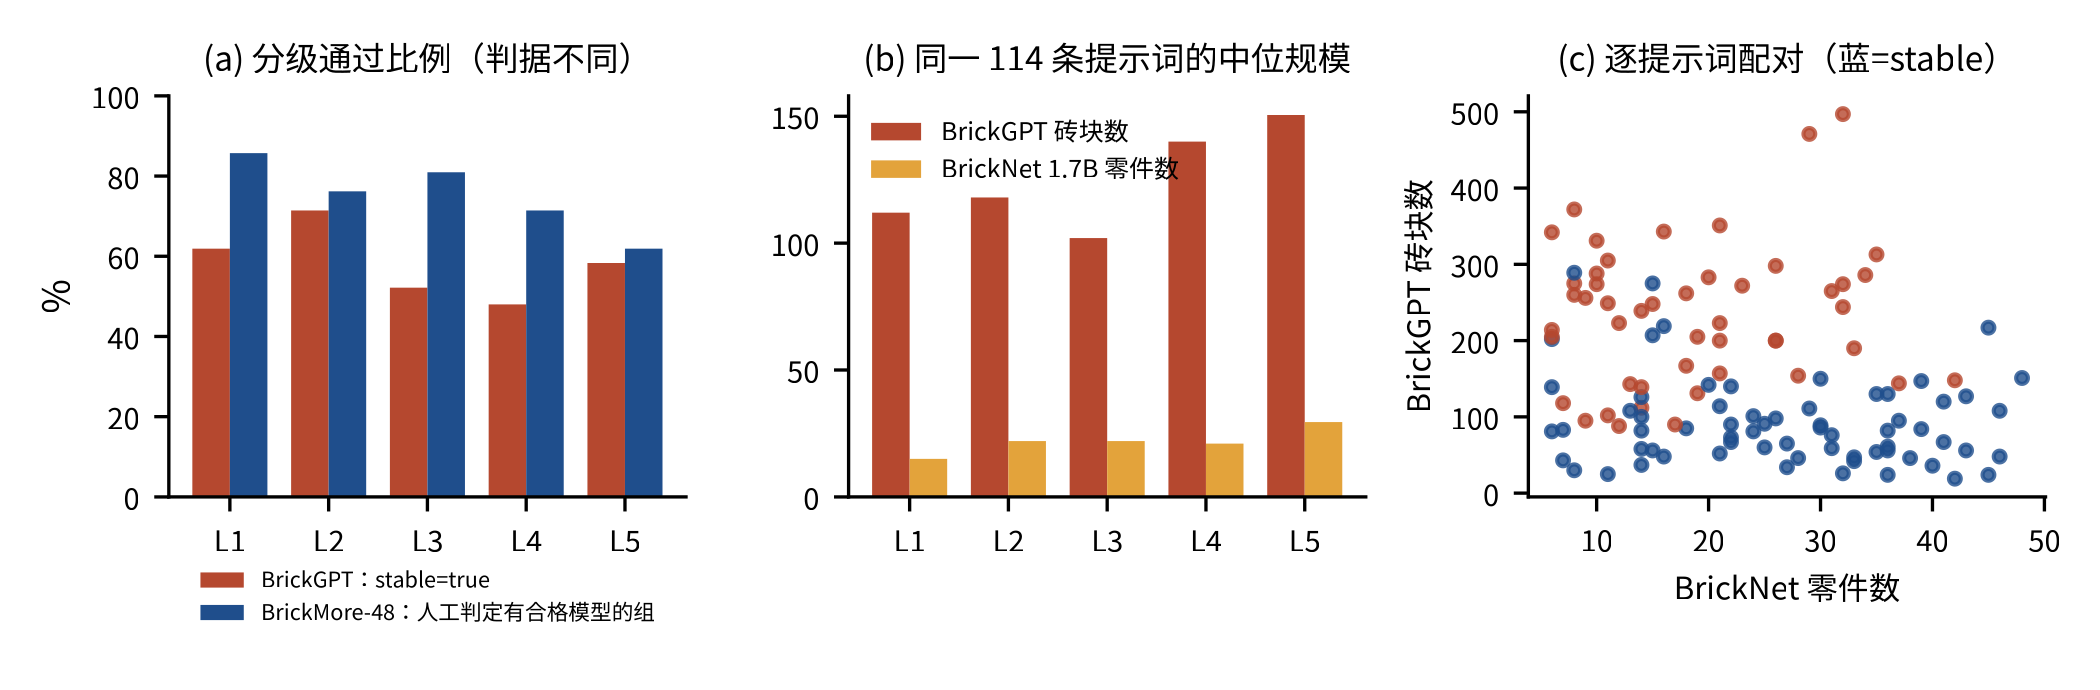
\includegraphics[width=0.88\textwidth,height=0.34\textheight,keepaspectratio]{figures/image18.png}\\[-0.3em]
\caption{Historical baseline comparison with differing acceptance criteria; not the current matched main comparison.}
\end{figure*}

\begin{figure*}[t]
\centering
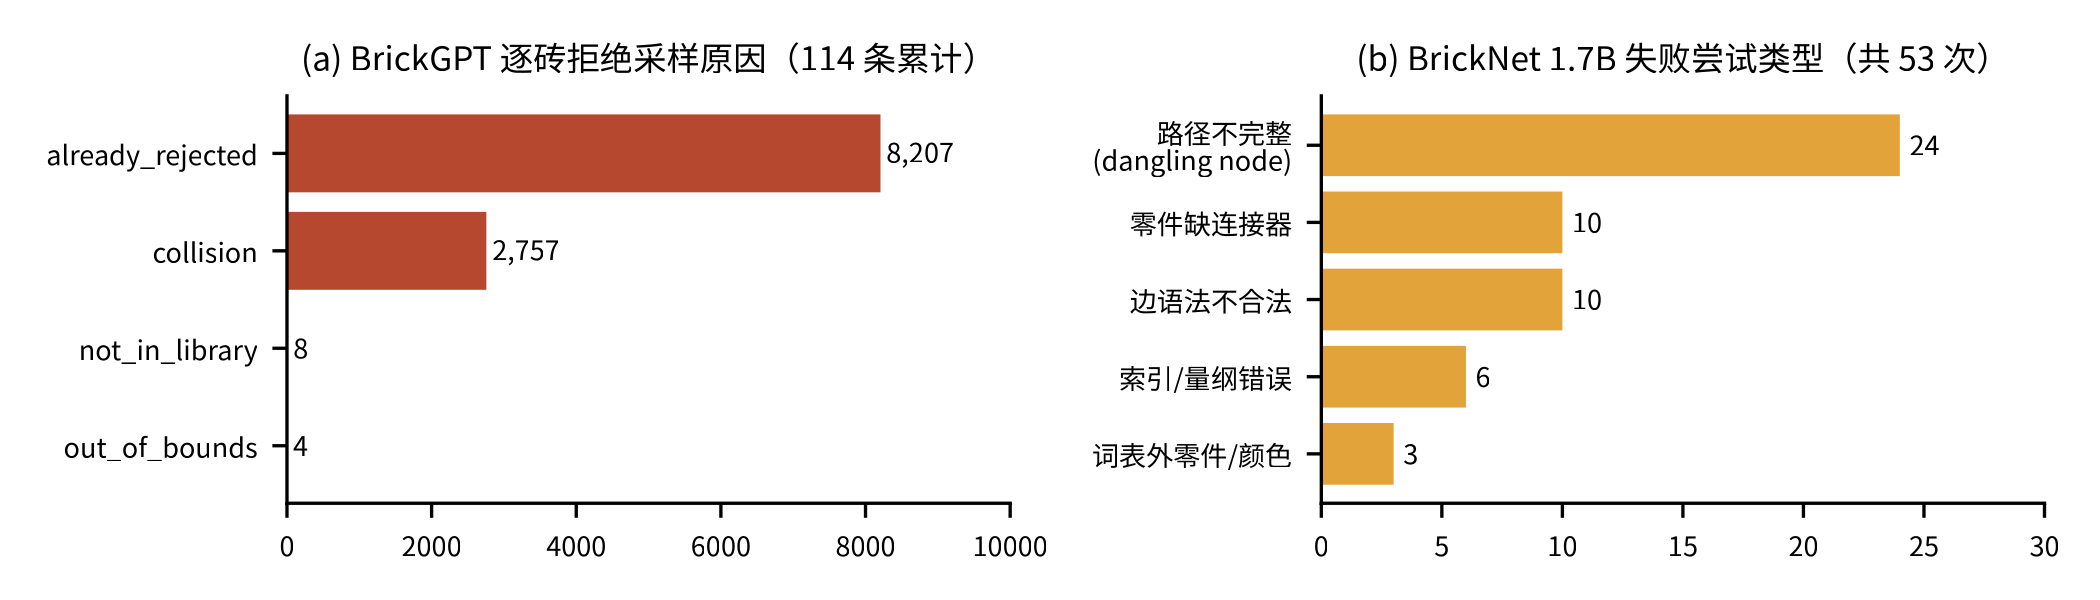
\includegraphics[width=0.88\textwidth,height=0.34\textheight,keepaspectratio]{figures/image19.png}\\[-0.3em]
\caption{Historical failure categories in the supplied reference; sample definitions require verification.}
\end{figure*}

\begin{figure*}[t]
\centering
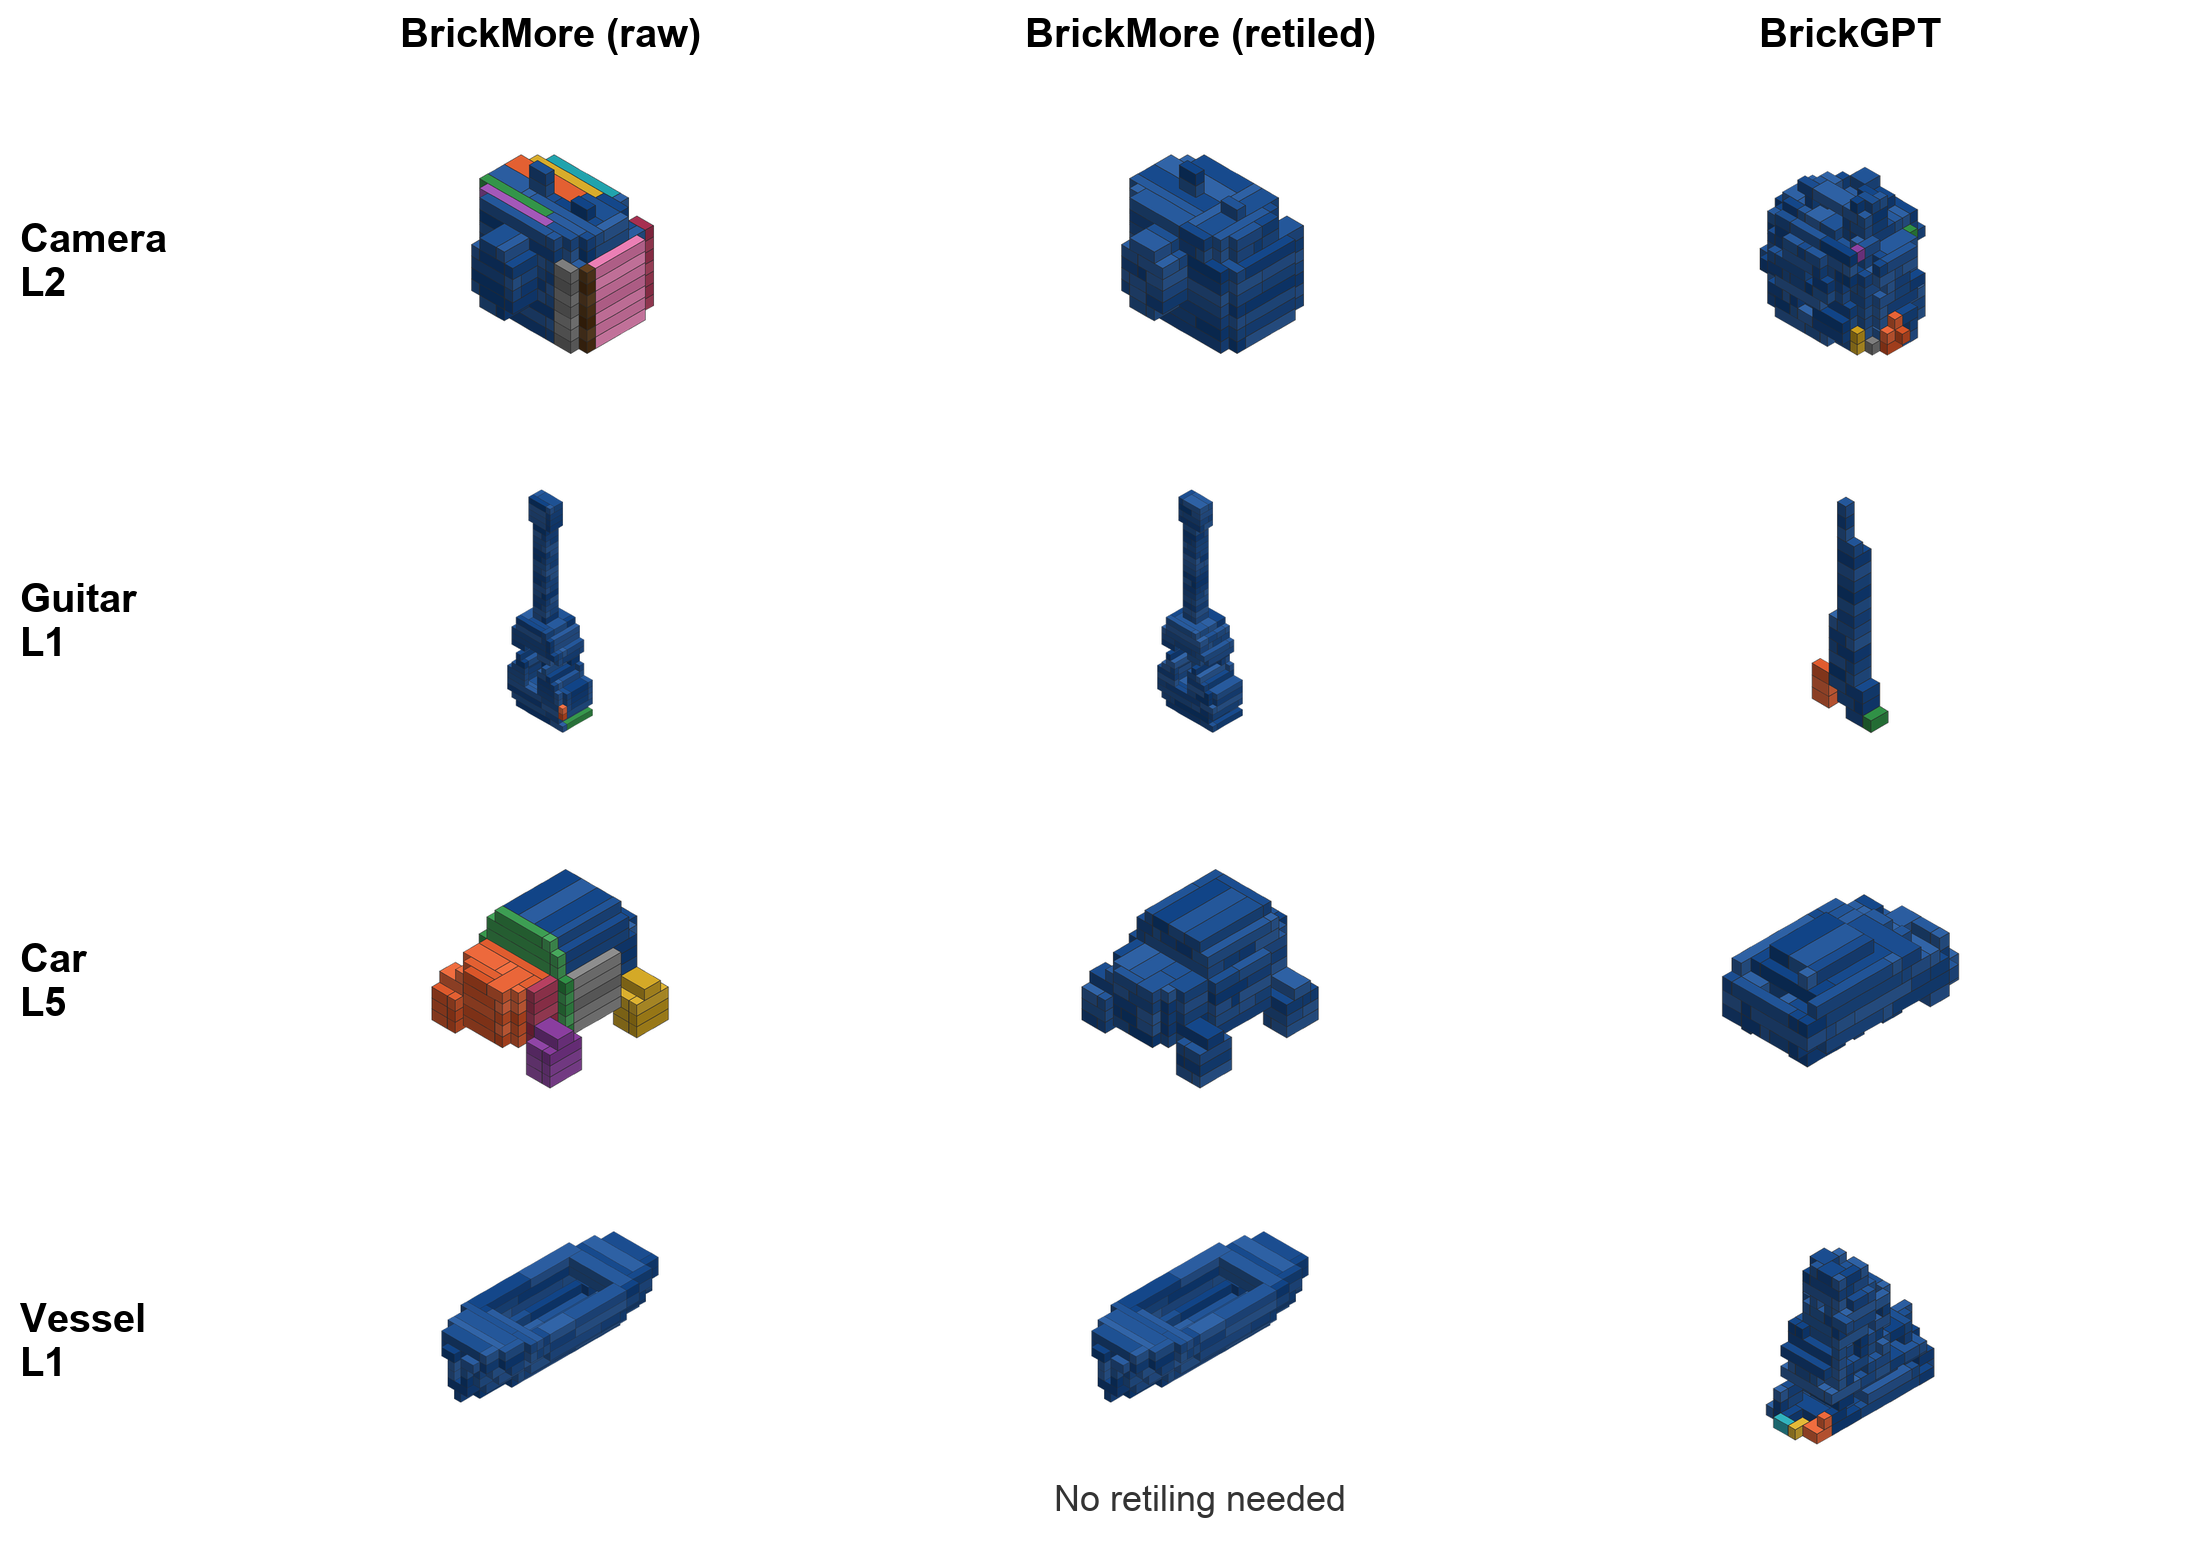
\includegraphics[width=0.88\textwidth,height=0.34\textheight,keepaspectratio]{figures/original_comparison.png}\\[-0.3em]
\caption{Qualitative historical examples from the supplied reference. Column labels distinguish raw BrickMore, retiled BrickMore, and BrickGPT outputs.}
\end{figure*}

\begin{figure*}[t]
\centering
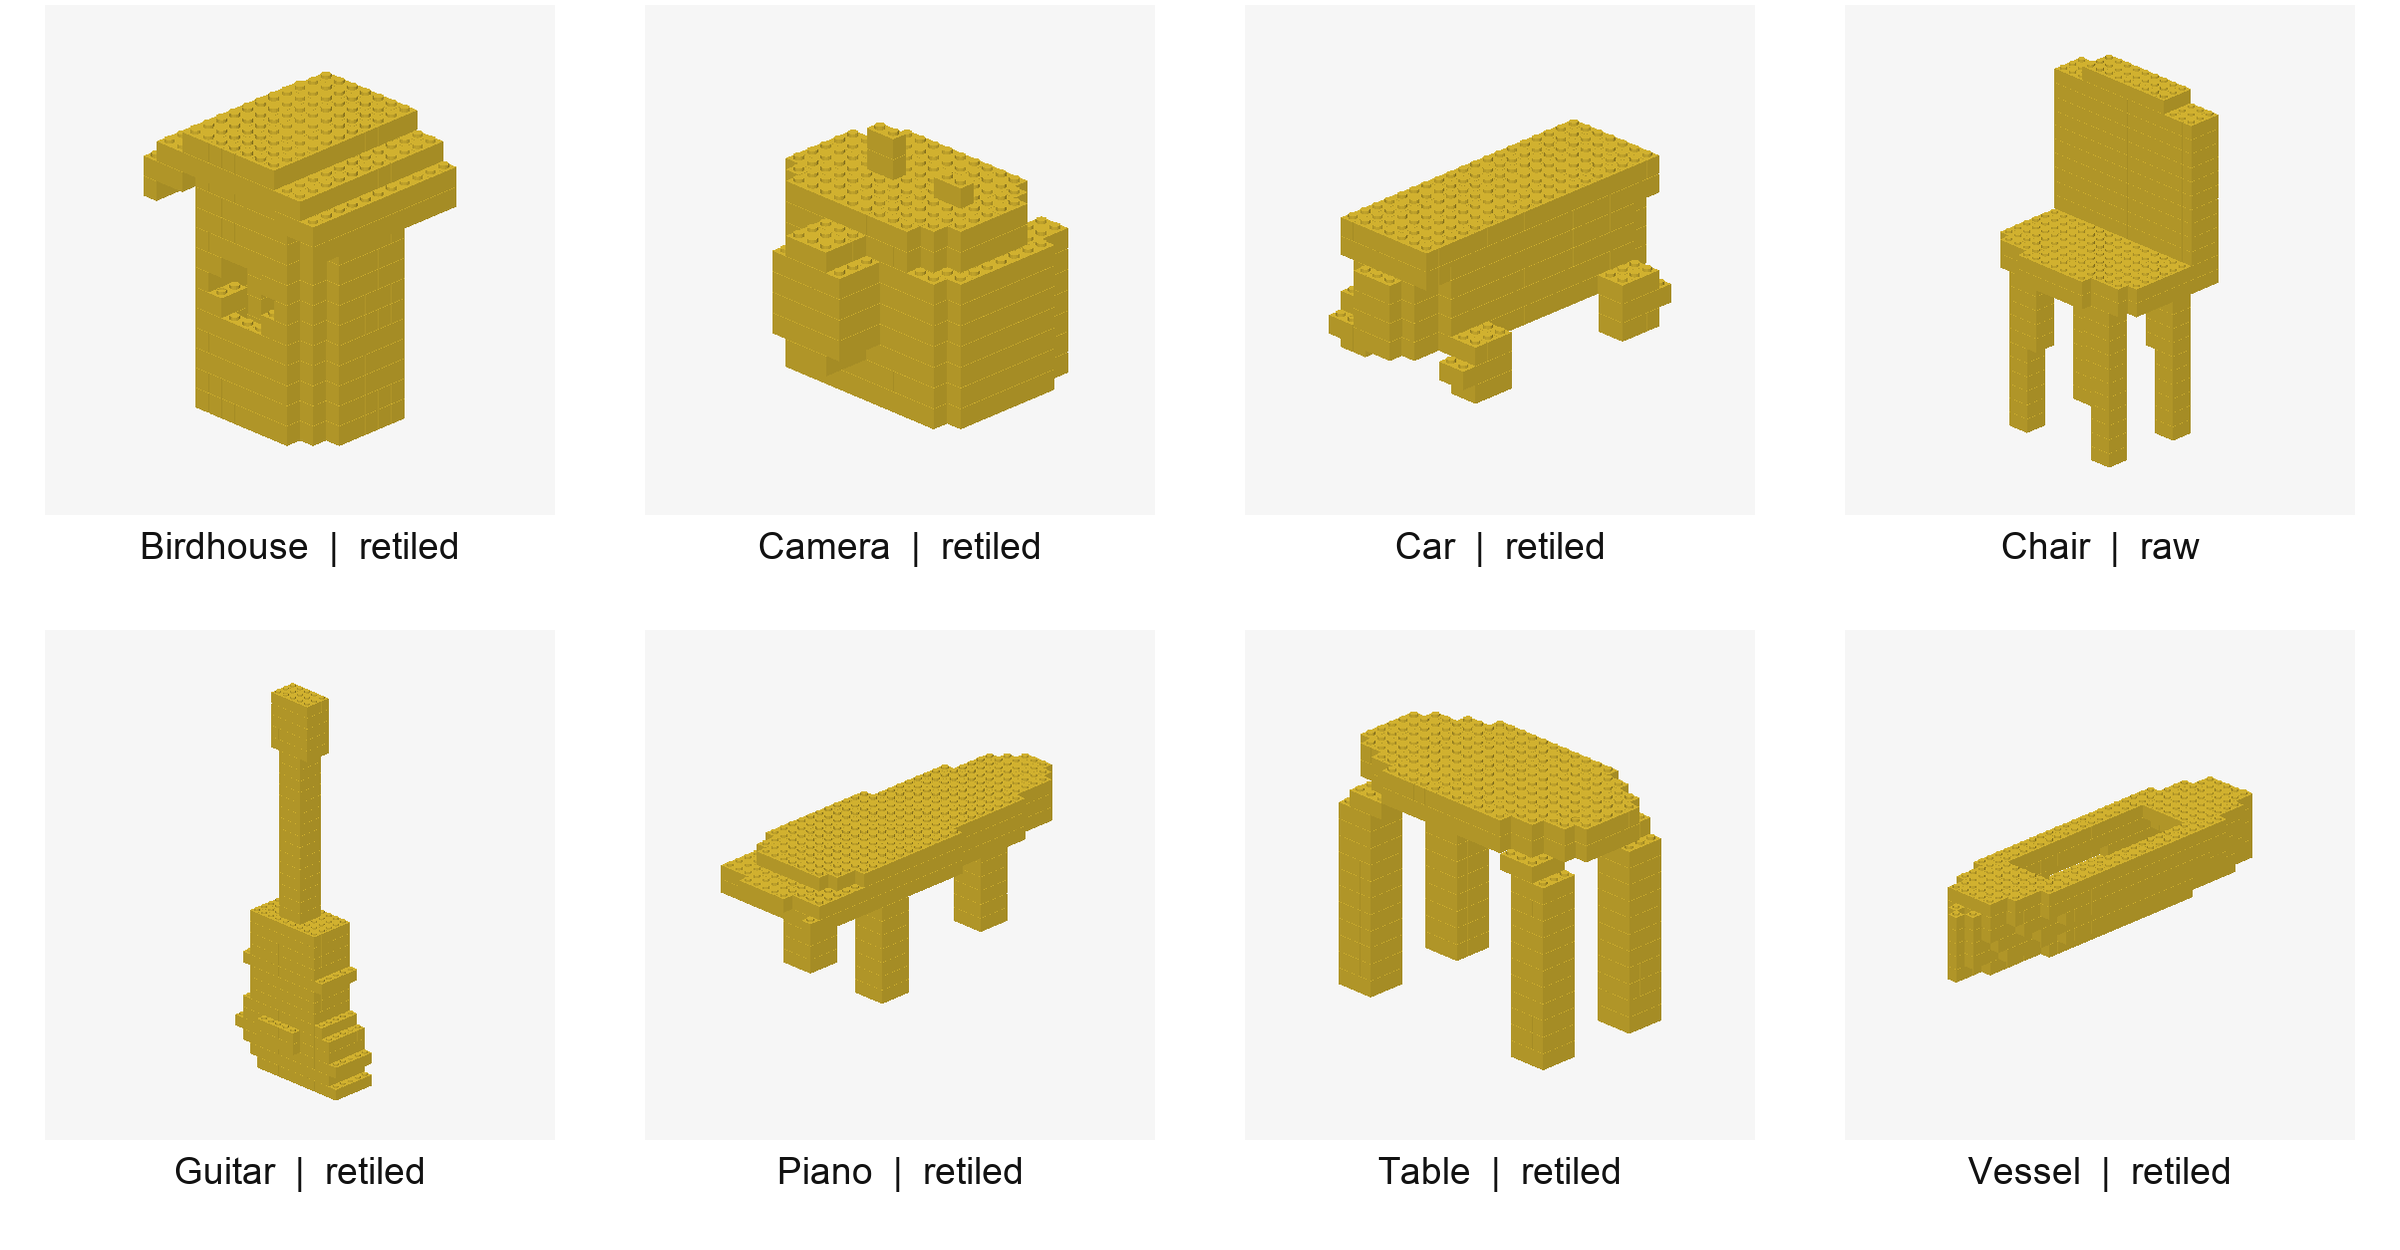
\includegraphics[width=0.75\textwidth,height=0.22\textheight,keepaspectratio]{figures/generated_gallery.png}\\[-0.3em]
\caption{Selected BrickMore outputs from the 114-prompt evaluation. One chair is raw; the other outputs are retiled. Results use uniform evaluation rendering and are not photographs of physical assemblies.}
\end{figure*}

\subsection{Raw and Stitched Outputs}
The supplied evaluation contains 110 matched raw and stitched BrickMore outputs. This paired subset is separate from the three-system main table. We match each pair by prompt, model identifier, and caption, and compare the mean scores before and after retiling.

\begin{table*}[t]\centering\small\begin{tabular}{lrr}\toprule
Metric & Raw & Stitched \\ \midrule
$P_{\mathrm{inv}}$ $\downarrow$ & 0.1897\% & 0.0000\% \\
VQAScore $\uparrow$ & 0.2065 & 0.2071 \\
PE $\uparrow$ & 0.1858 & 0.1859 \\
SigLIP2 $\uparrow$ & 0.1379 & 0.1261 \\
\bottomrule\end{tabular}\caption{Paired raw and retiled results on 110 matched cases.}\end{table*}
The mean invalid-placement ratio decreases to zero after retiling. VQAScore and PE change only slightly, while the mean SigLIP2 score decreases. These are descriptive results for the matched subset and do not establish a general causal effect.

\subsection{Evaluation Boundaries}
PE truncates 25 of the 114 main-comparison prompts, and SigLIP2 truncates 29; the affected prompts are the same across the three systems for each metric. The evaluation uses a common yellow rendering and therefore does not assess original colors. A zero $P_{\mathrm{inv}}$ does not establish stud connectivity, physical stability, or assembly feasibility.

\section{Limitations and Discussion}
The integrated dataset count is derived from versioned release reports; Section~\ref{sec:training} describes the 79,301-model training corpus obtained from that accounting. Dataset conversion may permit multiple grounded components, and its validation uses six-neighbour connectivity, whereas post-generation retiling enforces a single stud-connected component. Physical screening is based on stated assumptions and does not replace calibrated clutch-strength measurement or physical assembly tests.

The comparative evaluation covers 114 prompts and the provided outputs. The systems differ in their candidate selection and post-processing, and some text is truncated by evaluation models. These conditions limit how broadly the reported scores can be interpreted. Further paired uncertainty analysis can be conducted on the existing per-prompt records.

\section{Conclusion}
We present BrickMore, a text-to-brick framework combining agentic batch generation of training data, language-model fine-tuning, and post-generation geometric repair. The dataset workflow converts programmatically generated voxel shapes into brick layouts, while the generation pipeline predicts placements from text and checks reconstructed layouts for coverage, overlaps, and stud connectivity. On 114 shared prompts, the evaluated BrickMore outputs achieve the highest means on three text--image metrics, while matching BrickGPT on mean invalid-placement ratio. The results should be interpreted under the stated evaluation and physical-screening boundaries.

\FloatBarrier
{\footnotesize
\begin{thebibliography}{9}
\bibitem{brickgpt} A. Pun, K. Deng, R. Liu, D. Ramanan, C. Liu, and J.-Y. Zhu. Generating physically stable and buildable brick structures from text. In \emph{ICCV}, 2025. \url{https://arxiv.org/abs/2505.05469}.
\bibitem{bricknet} P. Kulits and C. Schmid. BrickNet: Graph-backed generative brick assembly. In \emph{CVPR}, 2026. \url{https://arxiv.org/abs/2604.22984}.
\bibitem{stablelego} R. Liu, K. Deng, Z. Wang, and C. Liu. StableLego: Stability analysis of block stacking assembly. \emph{IEEE Robotics and Automation Letters}, 9(11):9383--9390, 2024. \url{https://doi.org/10.1109/LRA.2024.3414281}.
\end{thebibliography}}
\clearpage
\onecolumn
\appendix
\section{Historical Tables from the Supplied Reference}
The following transcribed tables preserve the historical reference material. They use different versions or evaluation criteria and are not substitutes for the current main comparison. Values, physical-screening coverage, and missing entries require verification. Dashes indicate missing entries in the supplied source.
\begin{table}[!htbp]\centering\small
\begin{tabular}{lr}\toprule
Item & Historical value \\ \midrule
Voxel models & 80,000 (40,000 per batch) \\
Categories / structural families & 21 / 40 per category \\
Grid / voxel count & $48^3$ / 750--1,250 \\
Prompt records & 400,000 (five bilingual records per model) \\
Uniqueness & 80,000 unique; 0 A/B duplicates \\
Overlap with historical hashes & 0 / 55,255 \\
Retile geometry passes & 79,298 (99.12\%) \\
Bricks in full preview & 12,718,389 \\
Final gravity equilibrium passes & 220 \\
Final and layer-prefix passes & 128 \\
\bottomrule\end{tabular}
\caption{Historical dataset statistics transcribed from the supplied reference. The geometry count refers to the old retile release, not the later integrated count. Verify the preview and physical-screening totals against version-matched reports.}
\end{table}

\begin{table}[!htbp]\centering\scriptsize
\begin{tabular}{llrrrrr}\toprule
Version & Connectivity & Voxel changes & Passes & Rate & Final & Final + prefixes \\ \midrule
Strict v3 & Single; support $\geq$10\%, overhang $\leq$2 & None & 7,902 & 9.88\% & -- & -- \\
Relaxed & Each component grounded & +428,278 / -38,230 & 65,503 & 81.88\% & 2,650 & 478 \\
Retile & Each component grounded & +228,582 / -125 & 79,298 & 99.12\% & 220 & 128 \\
\midrule
\multicolumn{7}{l}{Uniform 160-model sample (seed 38177); not full-dataset results} \\
Baseline & Single stud-connected component & None & 22 & 13.75\% & -- & -- \\
Q3 & Single stud-connected component & Added $\leq$2\% & 55 & 34.38\% & 8 & 2 \\
Q4 (sparse) & Single stud-connected component & Added + removed $\leq$2\% & 57 & 35.63\% & 8 & 2 \\
\bottomrule\end{tabular}
\caption{Historical conversion-strategy table from the reference. Full-dataset and 160-model sample rows use different scopes; connectivity rules also differ. Final and prefix columns report screening outcomes under the stated historical assumptions.}
\end{table}

\begin{table}[!htbp]\centering\small
\begin{tabular}{lrrr}\toprule
Item & BrickGPT & BrickNet 1.7B & BrickMore-48 \\ \midrule
Representation & $20^3$ bricks & Assembly graph & $48^3$ bricks \\
Criterion & stable & Parseable & -- \\
Passes & 66/114 & 114/114 & -- \\
Median parts & 126.5 & 22 & -- \\
Range & 19--497 & 6--48 & -- \\
Mean time (s) & 189.6 & -- & -- \\
\bottomrule\end{tabular}
\caption{Historical baseline table in the source reference. These criteria differ, and missing BrickMore entries were marked TODO. This is not the current matched four-metric main table.}
\end{table}

\begin{table}[!htbp]\centering\small
\begin{tabular}{lrrrrl}\toprule
Level & $n$ & BrickGPT stable & BrickGPT median bricks & BrickNet median parts & BrickMore-48 \\ \midrule
L1 & 21 & 13 & 112 & 15 & -- \\
L2 & 21 & 15 & 118 & 22 & -- \\
L3 & 23 & 12 & 102 & 22 & -- \\
L4 & 25 & 12 & 140 & 21 & -- \\
L5 & 24 & 14 & 150.5 & 29.5 & -- \\
\bottomrule\end{tabular}
\caption{Historical level-wise baseline table transcribed from the reference. The original BrickMore column was incomplete, and the other columns use different criteria.}
\end{table}

\begin{table}[!htbp]\centering\small
\begin{tabular}{lrrrr}\toprule
Method and source & $P_{\mathrm{inv}}$ & VQA & PE & SigLIP2 \\ \midrule
BrickGPT (literature, as transcribed) & 0.063 & 0.050 & 0.157 & 0.052 \\
BrickNet 1.7B (literature, as transcribed) & 0.260 & 0.593 & 0.282 & 0.631 \\
BrickGPT (114 prompts, historical placeholder) & -- & -- & -- & -- \\
BrickNet (114 prompts, historical placeholder) & -- & -- & -- & -- \\
BrickMore-48 (114 prompts, historical placeholder) & -- & -- & -- & -- \\
\bottomrule\end{tabular}
\caption{Original reference table with literature values and historical placeholders. Literature values use another evaluation set and must not be directly compared with the present 114-prompt results; the precise $P_{\mathrm{inv}}$ definition and direction require checking against the original publication.}
\end{table}
\FloatBarrier

\end{document}
